\documentclass[a4paper,12pt]{article}

\def\term{Fall}
\def\year{2024}
\def\lecturer{Huang} %Wei-Cheng Huang
\def\coursenumber{Math265}
\def\coursename{Real Analysis}

\makeatletter
\ifx \nauthor\undefined
  \def\nauthor{Kaifeng Lu}
\else
\fi

\makeatletter
\ifx \email\undefined
  \def\email{\href{klu15@u.rochester.edu}{klu15 at u dot rochester dot edu}}
\else
\fi

\title{\coursenumber \, \coursename \, Class Notes}
\author{Based on lectures by Prof. \lecturer \\\small Notes taken by \nauthor\\\small Errata: \,\email}
\date{\term\ \year}

\usepackage{amsmath}
\usepackage{amsfonts}
\usepackage{amssymb}
\usepackage{amsthm}
\usepackage{caption}
\usepackage{enumitem}
\usepackage{fancyhdr}
\usepackage[margin=1in]{geometry}
\usepackage{listings}
\usepackage{multicol,multirow}
\usepackage[hidelinks]{hyperref}
\usepackage{parskip}
\usepackage{tikz}
\usepackage{wrapfig}
\usepackage{mathtools}

% Theorems-renew
\theoremstyle{definition}
\newtheorem*{aim}{Aim}
\newtheorem*{axiom}{Axiom}
\newtheorem*{claim}{Claim}
\newtheorem*{corollary}{Corollary}
\newtheorem*{conjecture}{Conjecture}
\newtheorem*{definition}{Definition}
\newtheorem*{example}{Example}
\newtheorem*{exercise}{Exercise}
\newtheorem*{fact}{Fact}
\newtheorem*{law}{Law}
\newtheorem*{lemma}{Lemma}
\newtheorem*{notation}{Notation}
\newtheorem*{proposition}{Proposition}
\newtheorem*{question}{Question}
\newtheorem*{theorem}{Theorem}
\newtheorem*{assumption}{Assumption}

\newtheorem*{remark}{Remark}
\newtheorem*{warning}{Warning}

% Special sets
\newcommand{\C}{\mathbb{C}}
\newcommand{\N}{\mathbb{N}}
\newcommand{\Q}{\mathbb{Q}}
\newcommand{\R}{\mathbb{R}}
\newcommand{\Z}{\mathbb{Z}}
\newcommand{\F}{\mathbb{F}}
\newcommand{\neighbor}[2]{V_{#1}{(#2)}}

% Brackets
\newcommand{\abs}[1]{\left\lvert #1\right\rvert}
\newcommand{\norm}[1]{\left\lVert #1\right\rVert}
\newcommand{\highlight}[1]{\textit{\textbf{\underbar{#1}}}}
\newcommand{\bra}{\langle}
\newcommand{\ket}{\rangle}

%Sequence
\newcommand{\seq}[2]{(#1_{#2})}

%Abbv
\newcommand{\st}{\text{ s.t. }}
\newcommand{\limx}[2]{\lim_{x\rightarrow #1} {#2}}
\newcommand{\ds}{\displaystyle}

%RenewCommand
\renewcommand\qedsymbol{$\blacksquare$}

\hypersetup{
    colorlinks,
    citecolor=black,
    filecolor=black,
    linkcolor=black,
    urlcolor=black,
    pdfpagemode=FullScreen
}

%Figures
\newcommand{\sidefig}[2]{
  \begin{wrapfigure}{#1}{1.7\textwidth}
    \includegraphics[width=0.6\textwidth]{image/#2}
    \centering
  \end{wrapfigure}
}
\newcommand{\centerfig}[1]{
  \begin{figure}[h]
    \includegraphics[width=0.6\textwidth]{image/#1}
    \centering
  \end{figure}
}


%%%%%%%%%%%%%%%%%%%%%%
% Set up fancy header/footer
\pagestyle{fancy}
\fancyhead[LO,L]{\nauthor}
\fancyhead[CO,C]{\coursenumber \ - Lecture notes}
\fancyhead[RO,R]{Prof. \lecturer}
\fancyfoot[LO,L]{}
\fancyfoot[CO,C]{\thepage}
\fancyfoot[RO,R]{}
\renewcommand{\headrulewidth}{0.4pt}
\renewcommand{\footrulewidth}{0.4pt}
%%%%%%%%%%%%%%%%%%%%%%

\begin{document}
\maketitle

\newpage

\section{Preliminaries}

\newpage

\subsection{Sets and Functions}

\newpage

\subsection{Mathematical Induction}

\newpage

\subsection{Finite and Infinite Sets}

\newpage

\section{The Real Numbers}

\newpage

\subsection{The Algebraic and Order Properties of $\R$}

\newpage

\subsection{Absolute Value and the Real Line}

\newpage

\subsection{The Completeness Property of $\R$}


\newpage

\subsection{Applications of Supremum}

\newpage
\subsection{Intervals}

\newpage
\section{Sequences and Series}
\subsection{Sequences and their limits}

\begin{definition}[\textbf{Seuqence}]
    A \highlight{sequence of real numbers} is a \textit{function} from $\N$ to $\R$.
\end{definition}
\begin{center}
    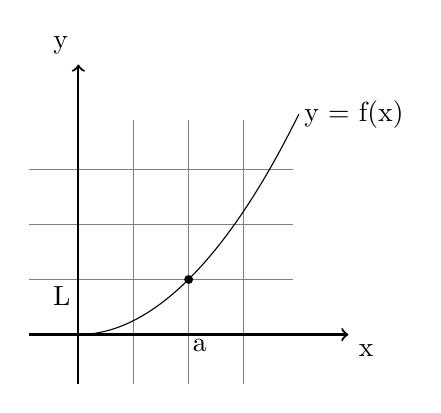
\begin{tikzpicture}[scale=0.7]
        \draw[step=1cm,gray,very thin] (-0.9,-0.9) grid (3.9,3.9);
        \draw[thick,->] (-0.9,0) -- (4.9,0) node[anchor=north west] {x};
        \draw[thick,->] (0,-0.9) -- (0,4.9) node[anchor=south east] {y};
        \draw (0,0) parabola (4,4);
        \draw (2.2,-0.2) node {a};
        \draw (-0.3,0.7) node {L};
        \draw (5,4) node{y = f(x)};
        \filldraw [black] (2,1) circle (2pt);
    s\end{tikzpicture}
\end{center}

We adopt the notation with a \textit{sequence}:
\[\,a:\N\rightarrow\R\]
where instead of writing \(a(1), a(2), \dots\), we write it as \(a_1, a_2, \dots\) which we called them 
\highlight{terms} or \highlight{elements} of the sequence.\\

\begin{notation}

\[(a_n)_{n=1}^\infty  \text{ or }  (a_n)_{n\in\N}  \text{ or }  (a_n)  \text{ or }  (a_n|n\in \N)\]\\
\end{notation}

\begin{definition}[\textbf{Converge to x}]
    A sequence \((x_n)\in\R\) \highlight{converges} to \(x\in\R\) if 
    \[\forall \epsilon >0,\, \exists N_\epsilon \in \N \text{ such that }n\ge N_\epsilon \rightarrow\abs{x_n - x} <\epsilon\]
    We write \[\lim_{n\to\infty}x_n = \lim_{n\to\infty}(x_n) = x\]\\
\end{definition}

\begin{definition}[\textbf{Convergent \& Divergent}]
    A sequence is \highlight{convergent} if it has a \highlight{limit} in \(\R\), and is \highlight{divergent} if it 
    has \highlight{no limit} in $\R$.\\
\end{definition}

\newpage
\begin{theorem}[\textbf{Uniqueness of Limit}]
    A sequence in $\R$ can have \highlight{at most one} limit. Or, the limit of a sequence is \highlight{unique} if the limit exists 
\end{theorem}
\begin{proof}
    Let \((x_n)\) be a sequence of real numbers. Suppose \(x,x'\) are limits of \((x_n)\). We want to prove \(x = x'\) by controdiction.
    \\\\Assume \(\abs{x-x'} > 0\). If we consider \(\epsilon := \frac{1}{3}\abs{x-x'}>0\), then\\
    \indent \(\text{The existence of } \lim_{x_n \to x}\text{implies that } \exists N_1 \in \N \text{ such that } \abs{x_n-x} < \epsilon\text{ if }n\ge \N_1. \)\\
    \indent \(\text{Similarly, existence of } \lim_{x_n \to x'} \text{implies that } \exists N_2 \in \N \text{ such that } \abs{x_n-x'} < \epsilon\text{ if }n\ge \N_2. \)\\
    Thus,
    \begin{align*}
        \abs{x-x'} & \le \abs{x-x_{N_1+N_2}+x_{N_1+N_2}-x'} & \\
                   & \le \abs{x-x_{N_1+N_2}}+\abs{x_{N_1+N_2}-x'} \text{ by triangle inequality}\\
                   & < \epsilon+\epsilon \\
                   & = \frac{2}{3}\abs{x-x'}
    \end{align*}
    Then, 
    \[\frac{1}{3}\abs{x-x'}<0,\text{which is a controdiction}\]
    we thereby prove by controdiction that
    \[\abs{x-x'} = 0\text{, which is equvalent to } x=x'\]
\end{proof}

\begin{example}
    \[\lim_{n\to \infty}(\frac{1}{n}) = 0\]
    Goal: \(\forall \epsilon>0,\) want to find \(N_\epsilon\) such that \(\abs{\frac{1}{n}-0} < \epsilon\) for \(n>N\), 
    so it suffices to show that \\
    \[\frac{1}{n}<\epsilon \Leftrightarrow \frac{1}{\epsilon} < n\]
\end{example}

\begin{proof}
    Let \(\epsilon>0\). Apply Archemedian's property to \(\frac{1}{\epsilon}\), then
    \begin{align*}
        & \exists N\in \N \text{ such that }\frac{1}{\epsilon}<N \\
        \Rightarrow & \forall n \ge N, \abs{\frac{1}{n}-0} = \frac{1}{n}\le \frac{1}{N} < \epsilon.\\
        \Rightarrow & \lim_{n \to \infty}\frac{1}{n} = 0
    \end{align*}
\end{proof}
\newpage
\begin{theorem}
    Let \((x_n)\) be a sequence of real numbers, and let \(x \in \R\). The following theorems are equvalent:
\begin{enumerate}
    \item \(x_n \rightarrow x\)
    \item \(\forall \epsilon > 0, \exists N \in \N \text{ such that } \abs{x_n-x}<\epsilon,\text{ for }n\ge \N \)
    \item \(\dots \dots x - \epsilon<x_n<x+\epsilon\dots\dots\)
    \item \(\forall\epsilon\text{-neighborhood } V_\epsilon(x),\exists N \in \N \text{ such that } x_n \in V_\epsilon(x) \text{ for } n\ge N\)\\
\end{enumerate}
\highlight{Sketch of proof:}
\[(1)\Leftrightarrow(2)\Leftrightarrow(3)\Leftrightarrow(4)\]
\end{theorem}

\begin{proposition}
    \[\lim_{n\to \infty}(2\sqrt{2n+1}-\sqrt{2n})=0\]
\end{proposition}

\begin{proof}
    Let \(\epsilon > 0\). Consider \[N = \lceil\frac{1}{2}(\frac{1}{2\epsilon})^2\rceil\in\N\]
    \[n>N\Rightarrow n>\frac{1}{2}(\frac{1}{2\epsilon})^2 \Rightarrow \frac{1}{2\sqrt{2n}}<\epsilon\Rightarrow\abs{\sqrt{2n+1}-\sqrt{2n}} = \dots = \frac{1}{\sqrt{2n+1}+\sqrt{2n}}<\epsilon\]
\end{proof}

\begin{remark}
    \[\lim_{n\to\infty}(-1)^n\text{ is undefined.}\]\\
\end{remark}

\begin{definition}[\textbf{m-tail}]
    If \((x_n)\) is a sequence of real numbers and \(m \in \N\), then the \highlight{m-tail} of \((x_n)\) is the sequence 
    \[\{x_{n+m}:n\in\N\}=\{x_{m+1}, x_{m+2}, \dots\}\]
\end{definition}

\begin{theorem}
    Let \((x_n)\) be a sequence and \(m\in\N\). Then \((x_n)\) is \highlight{convergent} iff \((x_{n+m})\) is \highlight{convergent}. 
    Moreover,\[\lim_{n\to\N}(x_n) = \lim_{n\to\N}(x_{n+m})\]
\end{theorem}

\begin{proof}
    \((\Rightarrow)\)\\
    Suppose \(x_n\to x\). Let\[\epsilon>0, \exists N_\epsilon >0, \text{ such that } \abs{x_n-x}<\epsilon \text{ for }n\ge N_\epsilon\]
    Consider \({N_\epsilon}':=N_\epsilon + m\) then
    \[n+m \ge {N_\epsilon}' \Rightarrow n\ge N_\epsilon \Rightarrow n+m\ge N_\epsilon \Rightarrow \abs{x_{n+m}-x}<\epsilon\]
    It follows that \[n\ge N_\epsilon \Rightarrow n+m \ge N_\epsilon \Rightarrow \abs{x_{n+m}-x}<\epsilon\]
    \newpage
    \((\Leftarrow)\)\\
    Suppose \(x_{n+m}\rightarrow x\).
    \[\forall \epsilon>0,\exists N_\epsilon>0 \text{ such that } \abs{x_{n+m}<\epsilon}, \forall n\ge N_\epsilon\]
    Consider \(N:=N_\epsilon+m\). Then 
    \begin{align*}
        & n\ge N = N_\epsilon+m \\
        & \Rightarrow n-m \ge N_\epsilon \\
        & \Rightarrow\abs{x_{(n-m)+m}-x}<\epsilon \\
        & \Rightarrow\abs{x_n-x}<\epsilon
    \end{align*}
\end{proof}

\begin{remark}
    We say that a sequence \((x_n)\) \highlight{ultimately} has a property if that property holds for some tail of \((x_n)\)\\
\end{remark}

\begin{theorem}
    Let \(x_n\) be a sequence of real numbers. 
    Let \(a_n\) be a sequence of positive real numbers such that \(\lim_{n\to \infty}a_n=0\).
    If \(\exists c>0, m\in \N, x\in \R\) such that \[\abs{x_n-x} \le c\cdot a_n,\forall n\ge m\]
    then \[x_n\to x\]
\end{theorem}

\begin{proof}
    We know that
    \[\forall \epsilon>0, \exists N\ge 0\text{ s.t. } \abs{a_n}<\frac{\epsilon}{c},\, \forall n\ge N\]
    Consider \(N'=max\{N,m\}, \forall n\ge N'\). Then 
    \[\abs{x_n-x}\le Ca_n = c\abs{a_n}<c\cdot\frac{\epsilon}{c} = \epsilon\]
    \[\Rightarrow x_n\rightarrow x\]
\end{proof}

\begin{proposition}
    \[\lim_{n\to\infty}\frac{17}{2+3n}=0\]
    \begin{proof}
        \[\abs{\frac{17}{2+3n}-0} = \frac{17}{2+3n} \le \frac{13}{3n} = \frac{17}{3}\cdot\frac{1}{n}\]
        Apply the theorem above with \[a_n=\frac{1}{n},c = \frac{17}{3}, m=1\]
        \[\Rightarrow\lim_{n\to\infty}\frac{17}{2+3n}=0\text{, since }\lim_{n\to\infty}\frac{1}{n}=0\]
    \end{proof}
\end{proposition}

\newpage
\begin{proposition}
    \[\forall c>0, \lim_{n\to\infty}c^{\frac{1}{n}}=1\]
    \begin{proof}

        \highlight{Case 1: c = 1} \[\lim_{n\to\infty}c^{\frac{1}{n}}=1\]
        \highlight{Case 2: c > 1}\\\\
        Let \(d_n = c^{\frac{1}{n}}-1\). Then \(\forall n, d_n>0\). It follows that 
        \begin{align*}
            (d_n+1)=c^{\frac{1}{n}} & \Rightarrow c= (1+d_n)^n\ge 1+n\cdot d_n\text{ by Bernoulli's inequality}\\
            & \Rightarrow d_n\le (c-1)\cdot \frac{1}{n} \\
            & \Rightarrow \abs{c^{\frac{1}{n}}-1} = d_n\le (c-1)\cdot\frac{1}{n}
        \end{align*}
        Apply the theorem with \[C = c-1,a_n = \frac{1}{n}, m=1,x=1\]
        \[\lim_{n\to\infty}c^{\frac{1}{n}}=1\]
        \highlight{Case 3: c < 1(Note that we cannot use Bernoulli inequality here)}\\\\
        Define \(e_n\) to be a sequence that satisfies \[c^{\frac{1}{n}} = \frac{1}{1+e_n}\]
        Then \(e_n>0\forall n\).
        \[c = \frac{1}{(1+e_n)^n}\le\frac{1}{1+n\cdot e_n} < \frac{1}{n\cdot e_n}\]
        \[\Rightarrow e_n < \frac{1}{c}\cdot \frac{1}{n}\]
        \[1-c^{\frac{1}{n}}= 1-\frac{1}{1+e_n}= \frac{e_n}{1+e_n}<e_n<\frac{1}{c}\cdot \frac{1}{n}\]
        Apply the theorem with \[a_n = \frac{1}{n}, m=1,C=\frac{1}{c}, x=1\]
        \[\lim_{n\to\infty} c^\frac{1}{n}=1\]
    \end{proof}
\end{proposition}

\newpage
\subsection{Limit Theorems}

\newpage
\subsection{Monotone sequence}

\begin{definition}
    Let \((x_n)\) be a sequence of real numbers
\end{definition}

\begin{theorem}[\textbf{Monotone Convergence Therorem}]
    A monotone sequence of real numbers is \highlight{convergent} iff it is bounded. 
Moreover, if \((x_n)\) is increaseing, then 
\[\lim(x_n) = \sup{x_n:n\in\N}\]
    If \((x_n)\) is decreasing, then 
    \[\lim(x_n) = \inf{x_n:n\in\N}\]\\
\end{theorem}

\begin{example}
    Consider the sequence \((x_n)\) is given by 
        \[\begin{cases}
            & x_0 = \frac{1}{2}\\
            & x_{n+1} = \frac{3}{2}x_n(1-x_n)\\
        \end{cases}\]

    \((x_n)\) is decreasing and  bounded.

    \highlight{Thoughts: } Assume \((x_n)\) converges, then by limit law,
    \[x = \frac{3}{2}x(1-x)\text{ where }x=\lim(x_n)\Rightarrow x = 0\text{ or }3\]
    then, by proof of controdiction, it is not convergent.
\end{example}

\begin{proof}
    \highlight{Claim}: \(\frac{1}{3}<x_{n+1}<x_n\le\frac{1}{2},\, \forall n \in \N \cup \left\{0\right\}\)\\\\
    \highlight{Proof of the claim by induction:} 

    When n = 0:
    \[x_0=\frac{1}{2},\, x_1 = \frac{3}{2}\cdot\frac{1}{2}(1-\frac{1}{2})=\frac{3}{8}\]
    \[\frac{1}{3}<\frac{3}{8}<\frac{1}{2}\le\frac{1}{2}\]

    Suppose this is true for n=k:
    \[\frac{1}{3}< x_{k+1}<x_k\le\frac{1}{2}\]

    Goal: \[\frac{1}{3}<x_{k+2}<x_{k+1}\le\frac{1}{2}\]
    \[x_{k+1} = \frac{3}{2}x_k(1-x_k)\]
    \[\frac{1}{3}<x_k\le\frac{1}{2}\,\Rightarrow\frac{2}{3}>1-x_k\ge\frac{1}{2}\]
    \[x_{k+1}<\frac{3}{2}\cdot\frac{1}{2}\cdot\frac{2}{3} = \frac{1}{2}\]
    Complete the square:
    \begin{align*}
        x_{k+1}-\frac{1}{3} & = \frac{3}{2}x_k(1-x_k)-\frac{1}{3}\\
        & = -\frac{3}{2}[(x_k-\frac{1}{2})^2-\frac{1}{36}]
    \end{align*}
    So
    \begin{align*}
        \frac{1}{3}<x_k\le\frac{1}{2}& \Rightarrow \abs{x_k-\frac{1}{2}}<\frac{1}{6}\\
        & \Rightarrow (x_k-\frac{1}{2})^2<\frac{1}{36}\\
        & \Rightarrow x_{k+1}-\frac{1}{3}>0\\
        & \Rightarrow \frac{1}{3}<x_{k+1}\le\frac{1}{2}
    \end{align*}
    With the similar process, we can derive that 
    \[\frac{1}{3}<x_{k+2}\le\frac{1}{2}\]
    \[x_{k+2} = \frac{3}{2}x_{k+1}(1-x_{k+1})<\frac{3}{2}x_{k+1}\cdot\frac{3}{2}=x_{k+1}\]
    Therefore, this claim is also true for n=k+1: \[\frac{1}{3}<x_{k+2}<x_{k+1}\le\frac{1}{2}\]
    We thereby prove the theorem by induction: 
    \[\frac{1}{3}<x_{n+1}<x_n\le\frac{1}{2}\]
\end{proof}

\highlight{Exercise: }
Textbook p.75: A sequence that converges to \(\sqrt{a}\) for \(a>0\).\newpage
\begin{definition}[\textbf{Euler's Number}]
    \[e = \lim(1+(\frac{1}{n})^n)\]
    \textbf{Goal: } \((x_n)\) is convergent where \(x_n=(1+\frac{1}{n})^n\)
    
    \begin{align*}
        x_n & = (1+\frac{1}{n})^n=1+nC1\cdot\frac{1}{n}+nC2\cdot\frac{1}{n^2}+\dots+nCn\frac{1}{n^n}\\
        & = 1+\frac{n}{1}\cdot\frac{1}{n}+\frac{n(n-1)}{2}\cdot\frac{1}{n^2}+\dots+\frac{n(n-1)\cdot3\cdot2\cdot1}{n!}\cdot\frac{1}{n^2}\\   
        & = 1 + 1+\frac{1}{2}(1-\frac{1}{n})+\frac{1}{6}(1-n)(1-\frac{2}{n})+\dots+\frac{1}{n!}(1-\frac{1}{n})(1-\frac{2}{n})\dots\frac{2}{n}\cdot\frac{1}{n}
    \end{align*}
    Write \(x_{n+1}\) in a similar way, we obserbe that \[x_n < x_{n+1}\]
    \highlight{Facts} \(2^{m-1}\le m!\) for \(m \in \N\Rightarrow \frac{1}{m!}\le\frac{1}{2^{m-1}}\)
    \[x_n<1+1+\frac{1}{2}+\frac{1}{4}+\dots+\frac{1}{2^{n-1}} = 1+\frac{1(1-(\frac{1}{2})^n)}{1-\frac{1}{2}}<3\]
    \(\Rightarrow(x_n) \)\text{ is increasing and bounded}
\end{definition}

\newpage

\subsection{Subsequence and the Bolzono-Weierstress Theorem}
    \begin{example}
        \begin{align*}
            (x_n) &= ((-1)^n)\\
            x_{2n} &= (-1)^{2n}\\
            x_{2n+1} &= (-1)^{2n-1}
        \end{align*}
        So \(a_n = x_{2n}\) is a sequence, while \(b_n = x_{2n+1}\) is a subsequence of \(x_n\).
    \end{example}

    \begin{definition}[\textbf{Subsequences}]
        Let \((x_n)\) be a real sequence and consider a strickly increasing seuqence of natural numbers 
        \(n_1<n_2<n_3<\dots\)
        . The sequence \[x_{n_k}\,:\,k\in\N\]
        is call a \highlight{subsequence} of \((x_n)\)
    \end{definition}
    \begin{example}
        Any tails of a squence is a subsequence:
        \((x_n)\) n-th dail: \((x_{m+k})\) is a subsequence
    \end{example}

    \begin{theorem}
        Suppose \((x_n)\) converges to \(x\). Then \(x_{x_k}\rightarrow x\) for any subsequence of \((x_n)\).
    \end{theorem}
    \begin{proof}
        Let \(\epsilon > 0\)
        \[\exists N_\epsilon >0 \text{ s.t. } \abs{x_n-x} < \epsilon \text{ for }n>N_\epsilon.\]
        Note that \[n_k \ge k,\,\forall k \in \N .\]
        The proof of the observation is exercise:
        \begin{exercise}
            By induction, \(n_1\ge 1, n_2 \ge n_1 \ge 1 \Rightarrow n_2 \ge 2\)
        \end{exercise}
        When \(k>N_k,\, n_k>N_\epsilon,\)
        \[\Rightarrow\abs{x_{n_k}-x}<\epsilon\]
        Therefore\[(x_{n_k})\rightarrow x\]
    \end{proof}

    \begin{theorem}
        Let \((x_n)\) be a sequence of real numbers, and let \(x\in \R\). Then the following are equvalent:
        \begin{enumerate}
            \item \((x_n)\) does not converge to \(x\).
            \item \(\exists \epsilon_0 >0, \text{ s.t. } \forall k \in \N, \exists n_k \in \N \text{ s.t. }\) 
            \[n_k\ge k\, \&\, \abs{x_{n_k}-x}>\epsilon_0\]
            \item \(\exists \epsilon_0 >0 \) \& a subsequence \(x_{n_k}\) s.t. \[\abs{x_{n_k}-x}>\epsilon_0,\, \forall k \in \N\]
        \end{enumerate}
    \end{theorem}
    \begin{proof}
        \begin{align*}
            3\rightarrow1 &\text{: by the contropositive statment of definition} \\
            3\rightarrow2 &\text{: 3 is a stronger statement of 2} \\
            1\rightarrow2 &\text{: left as exercise}
        \end{align*}
    \end{proof}
    \begin{theorem}
        If \(x_n\) satisfies either of the following property if it is \textbf{divergent}:
        \begin{itemize}
            \item There exists two subsequence \((x_{n_k})\) \& \((x_{m_k})\) whose limits are NOT equal.
            \item \((x_n)\) is unbouded.
        \end{itemize}
    \end{theorem}
    \begin{example}
        \text{\\}
        \begin{enumerate}
            \item \((-1)^n\)
            \item \((n)\)
            \item \((x_n)\) such that \[x_{2k} = k\]\[x_{2k+1} = (-1)^k\]
        \end{enumerate}
    \end{example}
    \begin{proof}
        \textit{exercise}\\
    \end{proof}

    \begin{theorem}[\textbf{Bolzano-Weierstrass Theorem}]
        A boudned sequence of real numbers has a \highlight{convergent subsequence}.
        \begin{example}
            \[x_n = (-1)^n\]
        \end{example}
        \begin{proof}
            \begin{lemma}
                If \((x_n)\) is a sequence of real numbers, there exists a subsequence of \((x_n)\) which is monotone.
            \end{lemma}
            \highlight{proof of lemma:}\\
            Call the m-th term \(x_m\) a \textit{"peek"} if \(x_m\) is at least as large as any term after it in the sequence.
            
            \begin{center}
                \begin{tikzpicture}
                    \draw[step=1cm,gray,very thin] (-0.9,-0.9) grid (3.9,3.9);
                    \draw[thick,->] (-0.9,0) -- (4.9,0) node[anchor=north west] {x};
                    \draw[thick,->] (0,-0.9) -- (0,4.9) node[anchor=south east] {y};
                    \filldraw [black] (1,1) circle (2pt);
                    \filldraw [black] (2,2) circle (2pt);
                    \filldraw [black] (3,1.5) circle (2pt);
                    \draw (3,1) node {"peek"};
                \end{tikzpicture}
            \end{center}

            \highlight{Case 1: }\((x_n)\) has infinitelyy many peaks

            List the peaks of \((x_n)\) in order of increasing index \[x_{n_1},x_{n_2},\dots\]
            \(\Rightarrow (x_{n_i})\) is a decreasing sequence.

            \highlight{Case 2: }\((x_n)\) has a finite number of peaks

            Let \(s_1\) be the first index after the last peak of \((x_n)\). Then for every \(n\ge s_1, \,\exists m\in\N\) such that \(x_m>x_n\).

            Choose \[s_2\ge s_1\text{ such that } x_{s_2}>x_{s_1},\, s_2\ge s_1\text{ such that } x_{s_2}>x_{s_1},\dots\]
            \[\Rightarrow (x_{s_i}) \text{ is an increasing sequence.}\]
            \begin{remark}
                Lemma + monotone convergent theorem implies Bolzano-Weierstrass theorem.
            \end{remark}

            \highlight{Second proof}

            Suppose \((x_n)\) is a bounded sequence.
            \[\Rightarrow \exists I_1=[a_1,b_1] \text{ such that }(x_n)\in I_1\]
            
            Consider \[I_2' = [a_1,\frac{a_1+b_1}{2}], \, I_2'' = [\frac{a_1+b_1}{2}, b_1]\]
            
            Let \(I_2 = [a_2,b_2]\) be one of \(I_2',I_2''\) such that \(I_2\) contains infinitely many terms of \((x_n)\).
            
            For \(n\in\N\), define \(I_n = [a_n,b_n]\) in a similar way.

            For \(i\in\N\), choose a term \(x_{n_i}\) such that \(x_{n_i}\in I_i\) and \(n_i>n_{i-1}\)

            Then \begin{align*}
                & i = 1,\, & n_i = 1\\
                & i = 2,\, & \text{choose }n_2\in\N \text{ such that } n_2>n_1 \,\& \,x_{n_2}\in I_2\\
                & \vdotswithin{=}\notag & \vdotswithin{=}\notag
            \end{align*}

            \begin{itemize}
                \item \(\forall i \in\N,\,a_i\le x_{n_i}\le b_i\)
                \item \((a_i) \text{ increases, bounded above by }b_1\Rightarrow (a_i)\rightarrow\sup{(a_i)}\)
                \item \((b_i) \text{ decreases, bounded below by }a_1\Rightarrow (b_i)\rightarrow \inf{(b_i)}\)
                \item \(\inf{\abs{a_i-b_i}} = \inf{\frac{b_1-a_1}{2^n}} = 0 \Rightarrow \sup{(a_i)} = \inf{(b_i)}\)
            \end{itemize}

            Thus \((x_{n_i})\) is convergent by squeeze theorem.\\
        \end{proof}
    \end{theorem}

    \begin{theorem}
        Let \((x_n)\) be a bounded sequence, and \(x\in\R\) has the property that every convergent subsequence of \((x_n)\) converges to \(x\). 
        Then \(x_n \text{ converges to } x\)
        \begin{proof}
            Let \(\forall\epsilon>0\)

            By Bolzano-Weierstrass theorem, \(\exists\) a convergent subsequence \((x_{n_i})\) such that
            \[\exists N_\epsilon\in\N \text{ s.t. for } i>N_\epsilon, \abs{x_{n_i}-x}<\epsilon\]
            
            Assume \((x_n)\) does not converge to \(x\). Then by previous theorem of subsequence,
            \[\exists \epsilon_0 >0 \text{ and a subsequence }(x_{n_k}) \text{ s.t. }\abs{x_{n_k}-x}>\epsilon_0, \forall k\in\N\]
            
            Since \((x_n)\) is bounded, \((x_{n_k})\) is also bounded. Thus there exists a convergent subsequence of \((x_{n_k})\) as \((x_{n_{k_i}})\).

            Note that \((x_{n_{k_i}})\) is a convergent subsequence of \((x_n)\), thus 
            \[(x_{n_{k_i}})\rightarrow x\text{ which is controdiction to previous assumption}\]
        \end{proof}
    \end{theorem}
    \begin{definition}
        Let \((x_n)\) be a sequence of real numbers. A point is called a \highlight{subsequential limit} of \((x_n)\) if it is the limit of a subsequence of \((x_n)\).
        \[S = \{\alpha \in\R:x\text{ is a subsequential limit}\}\text{ (NOTE: may be infinite set)}\]
        \begin{example}
            Consider \(\seq{x}{n}=\{(-1)^n|n\in\N\}\). Then 
            \[S \supseteq \{1,-1\}\]
        \end{example}

    \end{definition}

    \begin{definition}
        Let \((x_n)\) be a sequence of real numbers.
        \begin{itemize}
            \item The \highlight{limit superior} of \((x_n)\) is the infimum of the set of \(v\in\R\) s.t. \(v< x_n\) for at most a finite number of \(n\in\N\). We write it as
            \[\limsup(x_n) = \limsup x_n = \overline{\lim}x_n = \inf{\{v\in\R|v<x_n \text{ for at most a finite number of n}\}}\]
            \begin{example}
                Consider \(\seq{x}{n}=\frac{1}{n}\)
                \begin{center}
                    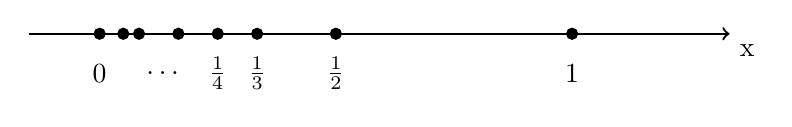
\begin{tikzpicture}
                        \draw[thick,->] (-0.9,0) -- (8,0) node[anchor=north west] {x};
                        \filldraw[black] (0,0) circle (2pt);
                        \draw (0,-0.5) node{0};
                        
                        \filldraw[black] (6,0) circle (2pt);
                        \draw (6,-0.5) node{1};
    
                        \filldraw[black] (3,0) circle (2pt);
                        \draw (3,-0.5) node{\(\frac{1}{2}\)};
    
                        \filldraw[black] (2,0) circle (2pt);
                        \draw (2,-0.5) node{\(\frac{1}{3}\)};
    
                        \filldraw[black] (1.5,0) circle (2pt);
                        \draw (1.5,-0.5) node{\(\frac{1}{4}\)};
    
                        \filldraw[black] (1,0) circle (2pt);
    
                        \filldraw[black] (0.5,0) circle (2pt);
    
                        \filldraw[black] (0.3,0) circle (2pt);
                        \draw (0.8,-0.5) node{\(\dots\)};
    
                    \end{tikzpicture}
                \end{center}

                Let\[X=\{v\in\R|v<x_n \text{ for at most a finite number of n}\}\]
                \begin{itemize}
                    \item \(-1\notin X\) because there are infinitely many \(x_n\) such that \(v<x_n\).
                    \item \(\frac{1}{2}\in X\) becasue there are finitely many \(x_n\) such that \(v<x_n\).
                    \item \(2\in X\) because there is no \(x_n\) such that \(v<x_n\), which is smaller than finite and thereby satisfies the definition.
                \end{itemize}

                We thus conclude that \[(0,\infty)\subset X\text{ and } \limsup{x_n} = \inf{X}\]
            \end{example}

            \begin{example}
                Consider \(\seq{x}{n} = (-1)^n\):
                \begin{center}
                    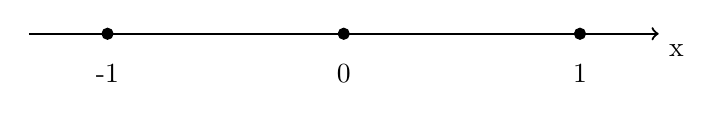
\begin{tikzpicture}
                        \draw[thick,->] (-4,0) -- (4,0) node[anchor=north west] {x};
                        \filldraw[black] (0,0) circle (2pt);
                        \draw (0,-0.5) node{0};
                        
                        \filldraw[black] (3,0) circle (2pt);
                        \draw (3,-0.5) node{1};
    
                        \filldraw[black] (-3,0) circle (2pt);
                        \draw (-3,-0.5) node{-1};
    
                    \end{tikzpicture}
                \end{center}
                \begin{itemize}
                    \item \(1\in X\) because there is no \(x_n\) such that \(v<x_n\).
                    \item \(2\in X\) because there is no \(x_n\) such that \(v<x_n\).
                    \item \(0,-1\notin X\) becasue there are infinitely many \(x_n\) such that \(v<x_n\).
                \end{itemize}
                We thus conclude that \[[1,\infty)\subset X\text{ (in fact they are equal)}\]
            \end{example}
            \item The \highlight{limit inferior} of \((x_n)\) is the supremum of the set of \(w\in\R\) s.t. \(w >x_m\) for at most a finite number of \(n\in\N\). We write it as
            \[\liminf(x_n)\text{ or }\liminf x_n\text{ or }\overline{\lim}x_n = \sup{\{w\in\R|w>x_n\text{ for at most a finite number of n}\}}\]
        \end{itemize}
    \end{definition}
    
    \highlight{Intuition} 

    \begin{itemize}
        \item Suppose \(v<x_n\) for at most finitely many \(n\in\N\), then for all large n, \(v\ge x_n\). \\\(\Rightarrow\) No subsequential limit of \(\seq{x}{n}\) can possibly exceed v.
        \item Similar observation for \(\underline{\lim{}}x_n\)\\
    \end{itemize}


    \begin{theorem}
        Let \((x_n)\) be a bounded sequence of real numbers, and let \(x^*\in\R\). Then TFAE:
        \begin{enumerate}
            \item \(x^* = \limsup(x_n)\)
            \item If \(\epsilon>0\), there are at most a finite number of \(n\in\N\) s.t.
            \(x^*+\epsilon <x_n\), but infinitely many n for which \(x^* - \epsilon<x_n\)
            \item If \(u_m=\sup{\{x_n|n\ge m\}}\)(sup of (m-1)-th tail), then \(x*=\inf{\{u_m|m\in\N\}} = \lim{u_m}\)
            \item If \(S\) is the set of subsequential limits of \(x_n\), then \(x^*=\sup S\).\\
        \end{enumerate}

        \begin{remark}
            .
            \begin{itemize}
                \item \(u_m\) is decreasing.
                \item There is a similar such list of equivalent properties for \(\liminf\).\\
            \end{itemize}
        \end{remark}
    
        \begin{corollary}
            A bounded sequence \((x_n)\) is convergent iff \(\overline{\lim}x_n = \lim x_n\)
            \begin{proof}
                A direct result of the theorem:\[\overline{\lim}x_n=\sup{S} \text{ and } \underline{\lim}x_n=\inf{S}\]
            \end{proof}
        \end{corollary}

        \begin{proof}[Proof of thm. (a) \(\Rightarrow\) (b)]
            Let \(\epsilon >0\). Then
            \[x^*+\epsilon>x^* = X =\inf{\{v\in\R | v<x_n \text{ for at most a finite number of n.}\}}\]
            \[\Rightarrow \exists v\in\R \text{ s.t. } x^*\le v < x^*+\epsilon\]
            and there are only finitely mant n with \(v<x_n\).
            
            For any \(n\) for which \(x^*+\epsilon < x_n\), \(v<x_n\). Thus there are only finitely many such n.

            If \(x^*-\epsilon \notin X\), then there are infinityly many \(n\) such that \(x^* - \epsilon<x_n\)
        \end{proof}

        \begin{proof}
            
        \end{proof}

        \begin{proof}[Proof of thm. (b) \(\Rightarrow\) (c)]
            Fix \(\epsilon>0\).

            By (b), there are only finitely many n with \(x^*+\epsilon<x\).

            Take \(N\in\N\) large enough such that
            \begin{align*}
                &&x^*+\epsilon&\ge x_n&\forall n\ge N\\
                &\Rightarrow&x^*+\epsilon &\ge u_N\\
                &\Rightarrow&x^*+\epsilon &\ge \lim{u_n}\\
                &\Rightarrow&x^* &\ge \lim{u_m} &\forall n\ge N
            \end{align*}

            On the other hand, there are infinitely many n with \(x^*-\epsilon<x_n\le u_n\). Thus,
            \(\text{ there exists a subsequence of }u_n\text{, say }u_{n_k}\text{, satisfies}\)
            \begin{align*}
                x^*-\epsilon\le u_{n_k}
            \end{align*}
        \end{proof}
    \end{theorem}
\end{document}